\documentclass[paper=a4, parskip=half-]{scrartcl}
\usepackage[utf8]{inputenc}

\usepackage{amsmath}
\usepackage{mathtools}
\usepackage{amssymb} % more icons/symbols
\usepackage{hyperref} % for hyper links
\usepackage{graphicx}
\usepackage{enumitem} % for enumerations a), i)
\usepackage{tcolorbox} % for colorful boxes
\usepackage{algpseudocode} % for algorithms
\usepackage{algorithm}

\usepackage{geometry}
 \geometry{
 a4paper,
 left=20mm,
 right=20mm,
 top=20mm,
 bottom=30mm,
 }


\title{Approximations- und Online-Algorithmen}
\author{\texttt{thgoebel@ethz.ch}}
\date{ETH Zürich, FS 2022}

% Custom commands
\newcommand{\setzeroone}{\lbrace 0, 1 \rbrace} % => {0,1} (Notice the missing $$)
\newcommand{\binarystring}{\setzeroone^*}
\newcommand{\horizontaldivider}{\begin{center} \line(1,0){350} \end{center}}
\newcommand{\A}{\mathcal{A}}
\newcommand{\B}{\mathcal{B}}
\newcommand{\M}{\mathcal{M}}
\newcommand{\I}{\mathcal{I}}
\newcommand{\E}{\mathbb{E}}
\newcommand{\N}{\mathbb{N}}
\newcommand{\R}{\mathbb{R}}
\newcommand{\bigO}{\mathcal{O}}
\newcommand{\bigOstar}{\mathcal{O}^*}
\newcommand{\cost}{\text{cost}}
\newcommand{\dist}{\text{dist}}
\newcommand{\Time}{\text{time}}
\newcommand{\st}{\; | \;} % st = such that
\newcommand{\cl}{\; : \;} % cl = colon

% Defines the box to contain the main takeaways from a section that you should be able to explain
\newenvironment{takeaway}{
    \begin{tcolorbox}[colback=red!5!white, colframe=red!65!white, title=Konzepte]
    \begin{itemize}[leftmargin=1em]
    \setlength{\itemsep}{-0.2em}
}
{
    \end{itemize}
    \end{tcolorbox}
}


\begin{document}

\begin{titlepage}
\maketitle
\vspace{5cm}
\thispagestyle{empty}


\begin{abstract}
This documents is a \textbf{short} summary for the course
\textit{Approximations- und Online-Algorithmen} at ETH Zurich.
It is intended as a document for quick lookup, e.g. during revision,
and as such does not replace attending the lecture, reading the slides or reading a proper book.

We do not guarantee correctness or completeness, nor is this document endorsed by the lecturers.
Feel free to point out any errata, either by mail or on
\href{https://github.com/eth-cs-student-summaries/Approximations-und-Online-Algorithmen}{Github}.
\end{abstract}

\end{titlepage}

\tableofcontents
\listoffigures
%\listoftables

Credits: images are generally taken from the lecture scripts.
\newpage

\part{Approximations-Algorithmen}

\section{Approximations-Algorithmen}

TODO.
Siehe das \href{https://github.com/eth-cs-student-summaries/Algorithmik-fuer-Schwere-Probleme/}{Skript von letzem Jahr}.

\newpage

\section{Approximationsschemata}

\begin{takeaway}
    \item PTAS, FPTAS
    \item SKP: 2-Approximation (Greedy), PTAS-SKP
    \item KP: DPKP, FPTAS
\end{takeaway}

\paragraph{Definition PTAS und FPTAS}
Eingabe $(I, \varepsilon)$.
PTAS: Laufzeit ist polynomiell in $|I|$ und beliebig in $\varepsilon^{-1}$.
FPTAS: Laufzeit ist polynomiell in $|I|$ \underline{und} in $\varepsilon^{-1}$.
Approximationsgüte $(1+\varepsilon)$.
Siehe [ASP].

\paragraph{Einfaches Rucksackproblem (Simple Knapsack Problem SKP)}
Gewichte = Kosten. NP-schwer.
Siehe [ASP].

\paragraph{Greedy-SKP}
2-Approximation. Absteigend sortieren, $\bigO(n \log n)$.
Siehe [ASP].

\paragraph{PTAS-SKP}
$(1+\varepsilon)$-Approximation.
$k \gets \lceil \frac{1}{\varepsilon} \rceil$.
Optimale Lösung für alle $\bigO(n^k)$ Teilmengen der Grösse $k$. Dann greedy erweitern in je $\bigO(n)$.
Siehe [ASP].

\paragraph{Allgemeines Rucksackproblem (KP)}
Eingabe $I = (w_1, ..., w_n, c_1, ..., c_n, b)$.
Siehe [ASP].

\paragraph{Exakter Algorithmus für KP (DPKP)}
Dynamische Programmierung. Siehe [ASP].

Sei $I_i$ die Teilinstanz der ersten $i$ Elemente.
Berechne Tripel:
$$ (k, W_{i,k}, T_{i,k}) \in (0, ..., \sum c_j) \times (0, ..., b) \times Pot({1, ..., n})
    = \text{Nutzen} \times \text{Gewicht} \times \text{Teilmenge} $$
wobei $W_{i,k}$ für Nutzen $k$ minimal ist und $W_{i,k} \leq b$.
Sei $TRIPLE_i$ die Menge alle Tripel für $I_i$.

Iteriere über alle $i$, und alle $TRIPLE_i$, und erweitere die Tripel um das i-te Element.
Gebe das grösste $k$ aus allen gefundenen Tripeln aus.

Laufzeit: $\bigO(|I| \cdot \sum c_j) = \bigO(n \cdot n \cdot \text{max-int}(I)) \implies$ pseudopolynomiell

Falls $b \ll \sum c_j$: speichere Tripel für jedes mögliche Gewicht den maximalen Nutzen
(anstatt für jeden möglichen Nutzen das minimale Gewicht).

\paragraph{FPTAS-KP}
Siehe [ASP].

\begin{enumerate}
    \item $t \gets \frac{\varepsilon \cdot c_{max}}{(1+\varepsilon)\cdot n}$
    \item Runde $c_i' \gets \lfloor \frac{c_i}{t} \rfloor$
    \item DPKP auf gerundete Instanz
\end{enumerate}
Korrektheit: Lösung bleibt zulässig.
Approximationsgüte: messy, siehe Buch/[ASP].\\
Laufzeit: $\bigO (n + n \cdot \sum c_j') = \bigO (\frac{1}{\varepsilon}n^3)$
$\implies$ poly($n, \varepsilon^{-1}$)

\newpage

\input{3-reduktionen}
\newpage


\part{Online-Algorithmen}

\section{Das Paging-Problem}

\begin{takeaway}
    \item Online-Problem, Online-Algorithmus, kompetitiver Faktor
    \item Paging-Problem
\end{takeaway}

\paragraph{Motivation}
Probleme lösen ohne vollständige Informationen zu haben (die für eine optimale Lösung relevant sind).
Stattdessen werden die Informationen stückweise zur Laufzeit bekannt.

\paragraph{Online-Problem}
Ein \emph{Online-Minimierungsproblem} ist $\Pi = (I, O, cost, \min)$.
Eine Eingabe $I = (x_1, ..., x_n) \in \mathcal{I}$ ist eine Folge von \emph{Anfragen}.
Eine akzeptierte Lösung $O = (y_1, ..., y_n)$ ist eine Folge von \emph{Antworten}.

Beim analogen Maximierungsproblem spricht man statt von $cost(I, O)$ oft vom \emph{Gewinn} $gain(I,O)$.

\paragraph{Online-Algorithmus}
Sei $\Pi$ ein Online-Optimierungsproblem.
Ein \emph{Online-Algorithmus} $\A$ berechnet die Ausgabe $\A(I) = (y_1, ..., y_n) $
wobei $y_i$ nur von $(x_1, ..., x_i)$ abhängt.
$\A(I)$ ist eine zulässig Lösung für $I$.

\paragraph{Kompetitive Faktor}
(aka. competitive ratio, Wettbewerbsgüte, kompetitive Güte) \\
Ein Online-Algorithmus $\A$ ist \emph{c-kompetitiv} falls gilt:
\begin{align*}
\exists \alpha \geq 0 \quad \forall I \cl \quad cost(\A(I)) & \leq c \cdot cost(Opt(I)) + \alpha \\
\dfrac{cost(\A(I))}{cost(Opt(I))} + \alpha' & \leq c
\end{align*}
für ein Minimierungsproblem und $\alpha$ konstant.
$Opt$ ist ein optimaler Offline-Algorithmus, d.h. mit vollständiger Information.

Das kleinste $c$ für das dies gilt heisst \emph{kompetitiver Faktor}. \\
Für $\alpha = 0$ heisst $\A$ \emph{strikt-c-kompetitiv}. \\
Falls $\A$ strikt-1-kompetitiv ist ($\alpha = 0, c = 1$) so heisst er \emph{optimal}.

Ein Online-Algorithmus heisst \emph{kompetitiv} wenn sein kompetititver Faktor nicht von der
Länge der Eingabe abhängt.
Wir sprechen dabei von \emph{kompetitiver Analyse}.
Der kompetitiver Faktor ist vergleichbar mit der Approximationsgüte von Approximationsalgorithmen.

Die Konstante $\alpha$ ist wichtig da sie erlaubt auf kurze Eingaben schlecht zu sein
(und erst auf lange besser zu werden).
\footnote{Warum brauchen wir bei der Approximationsgüte keine vergleichbare Konstante?}

\paragraph{Paging}
\begin{itemize}
    \item Eingabe: $ I = (x_1, ..., x_n)$ mit Speicher-Indizes $x_i \in \N$
    \item Hauptspeicher mit $m$ Seiten: $ (s_1, ..., s_m) $
    \item Cache-Speicher mit $k$ Seiten: $ B = (s_{j_1}, ..., s_{j_k}) $, initialisiert mit $ (s_1, ..., s_k) $
        \footnote{Der Vorsprung eines selbstgewählten Startinhalts kann in $\alpha$ versteckt werden.}
    \item Zeitschritt $i$:
    \begin{itemize}
        \item Index $x_i$ wird angefragt
        \item Falls $x_i$ im Cache (d.h. $s_{x_i} \in B$): return $y_i=0$
        \item Andernfalls: return $y_i=j$, und setze $B = B \backslash  \{s_j\} \cup \{s_{x_i}\} $,
            d.h. lösche Seite $s_j$ aus dem Cache.
            \footnote{Zusätzliches, proaktives Entfernen bringt keinen Vorteil.}
    \end{itemize}
    \item $ cost(\A(I)) := \vert \{ i \st y_i > 0 \} \vert $
    \item goal := min
\end{itemize}

Strategien bei \emph{Seitenfehlern (page faults)} zum \emph{Verdrängen} von Seiten:
First-in-First-Out (FIFO, wie eine Queue),
Last-in-First-Out (LIFO, wie ein Stack),
Least-Recently-Used (LRU),
Longest-Forward-Distance (LFD, offline-only!).

\paragraph{Satz}
Ein Online-Algorithmus für Paging der FIFO nutzt ist strikt-k-kompetitiv.

\underline{Beweis:}
Gruppiere Zeitschritte in \emph{Phasen}.
Phase 1 endet nach dem ersten Seitenfehler.
Phase $P \geq 2$ endet nach $1+ (P-1)k$ Seitenfehlern, d.h. alle $k$ Fehler endet eine Phase und beginnt eine neue.

In Phase 1 machen $Opt$ und $Fifo$ je genau einen Fehler (warum?).

Sei $s$ die Seite die den letzten Seitenfehler von Phase $P-1$ verursacht
(d.h. sie kommt neu in den Cache, und wird dank FIFO als letztes in Phase $P$ verdrängt werden). \\
$\implies$ Zu Beginn von Phase $P$ ist $s$ im Cache von $Opt$ \underline{und} von $Fifo$. \\
$\implies$ Es gibt $\leq k-1$ Seiten die im Cache von $Opt$ sind, aber nicht in dem von $Fifo$. \\
Während Phase $P$ macht $Fifo$ genau $k$ Fehler. \\
$\implies$  Während $P$ muss $Opt$ mindestens einen Seitenfehler machen. \\
$\implies$  $Fifo$ ist k-kompetitiv.

LRU ist in der Theorie ebenfalls k-kompetitiv, in der Praxis allerdings tendenziell besser als FIFO.



\newpage

\section{k-Server-Problem}

\begin{takeaway}
    \item k-Server-Problem
    \item Potentialfunktionen, amortisierte Kosten
    \item Greedy, Double Coverage
\end{takeaway}

\paragraph{Motivation}
Bewege Objekte in einem Raum zu bestimmten Punkten.
Z.B. Polizisten von Dienststellen zu crime scenes, oder Taxis zu Kunden.

``Heiliger Gral'' der Online-Algorithmen, wie TSP für Approximations-Algorithmen oder SAT für NP.

\paragraph{Metrischer Raum}
Sei $S$ eine Menge von Punkten, sei $\dist : S \times S \mapsto \mathbb{R}$ eine Distanzfunktion.
$\mathcal{M}(S, \dist)$ ist ein \emph{metrischer Raum} falls gilt:
Definitheit, Symmetrie, Dreiecksungleichung.

Beispiel: Euklidischer Raum. Vollständige, gewichtete, ungerichtete Graphen mit Dreiecksungleichung.
\\
Beobachtung: Alle Graphen mit Kastenkosten $\in \{1, 2\}$ erfüllen die Dreiecksungleichung.

\paragraph{k-Server}
Sei $\mathcal{M}(S, \dist)$ ein metrischer Raum.
Sei $s_1, ..., s_k$ Server als Punkte in $S$.
Sei eine Multimenge $C_i \subseteq S$ mit $|C_i|=k$ eine \emph{Konfiguration} von Servern in Zeitschritt $i$.
\\
Die \emph{Distanz} \footnote{Achtung Verwechslungsgefahr!}
zwischen $C_r$ und $C_t$ sind die Kosten eines minimalen Matchings zwischen ihnen.

Eine Instanz $I = (x_1, ..., x_n)$ fragt Punkte an, so dass in Zeitschritt $i$ ein Server nach $x_i$
bewegt werden muss (falls dort noch keiner steht).

Ziel: $\min \sum_i costMinMatching(C_i, C_{i+1})$

\paragraph{Träge}
Ein Online-Algorithmus für k-Server heisst \emph{träge (lazy)} wenn er nur dann einen Server bewegt,
wenn auf $x_i$ noch kein Server steht.
Auch bewegt er pro Zeitschritt maximal einen Server.

Dies erleichtert die Analyse. Gleichzeitig gilt (Satz): \\
Jeder c-kompetitive OA für k-Server kann in einen trägen OA umgewandelt werden der auch c-kompetitiv ist.

\paragraph{k-Server als Verallgemeinerung von Paging}
Cache $k$, Hauptspeicher $m$ $\longrightarrow$ vollständiger Graph mit $m$ Knoten und initial
Servern auf $(v_1, ..., v_k)$. Angefragte Punkte = angefragte Seiten.

Daraus folgt eine untere Schranke (Satz):
Es existiert ein metrischer Raum so dass kein deterministischer OA für k-Server besser als k-kompetitiv ist.
\\
Frage: für Paging ist die Schranke scharf, d.h. wir kennen einen Algo (z.B. FIFO).
Können wir für k-Server auch einen Algo konstruieren?

\paragraph{k-Server Vermutung(en)}
\begin{itemize}
    \item Es existiert ein k-kompetitiver deterministischer OA für k-Server.
    \item Es existiert ein im Erwartungswert $\Theta(\log k)$-kompetitiver randomisierter OA für k-Server.
\end{itemize}
D.h. die untere Schranke ist erreichbar.
Wenn dies wahr ist, dann ist k-Server genauso schwer wie Paging!
Aktueller Stand: $2k-1$.

\paragraph{Greedy-Algorithmus}
Bewege immer den Server der am nähesten dran ist.

\underline{Satz:}
$Greedy$ ist nicht kompetitiv für k-Server.

\underline{Beweis:}
Siehe Instanz in \autoref{k-server-greedy}.
Hier gilt $\frac{cost(Greedy(I))}{cost(I)} = \frac{n}{2}$, d.h. es gibt keine Konstante $c$
so dass $Greedy$ $c$-kompetitiv wäre.

\begin{figure}[h]
    \centering
    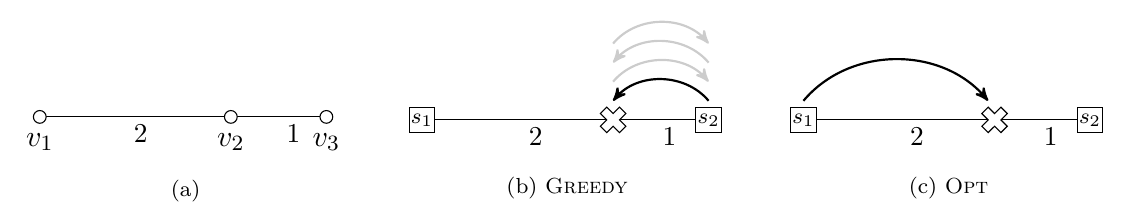
\includegraphics[width=0.8\textwidth]{images/k-server-greedy.png}
    \caption{k-Server: $Greedy$ versus $Opt$}
    \label{k-server-greedy}
\end{figure}


\subsection{Potentialfunktionen}

\paragraph{Motivation}
Kompetivität $c$ abschätzen über die \emph{amortisierten Kosten}.
Statt dass $cost(A(I)) \leq c \cdot cost(Opt(I)) + \alpha$ für alle $I$ gelten muss,
wollen wir zeigen dass $cost(A(x_i)) \leq c \cdot cost(Opt(x_i)) + \alpha$ für alle $x_i$ gilt.
\\
Dann können wir erlauben dass $A$ in einigen Zeitschritten mehr als $c$-mal schlechter ist als $Opt$,
solange er in anderen wieder weniger schlecht ist.

\paragraph{Potentialfunktion}
Sei $\mathcal{K}_{Alg}$ die Menge aller \emph{Konfigurationen} von $A$ auf Instanz $I$
und sei $\mathcal{K}_{Opt}$ die Menge aller Konfigurationen eines beliebigen, aber festen, $Opt$.
\footnote{Konfiguration: nach aussen sichtbar, nicht der interne state der Turingmaschine.
Z.B. Position der Server, Seiten im Cache.}

Dann ist eine \emph{Potentialfunktion} $\Phi$:
$$
\Phi \cl  \mathcal{K}_{Alg} \times \mathcal{K}_{Opt} \mapsto \R
\qquad \text{oder} \qquad
\Phi \cl \I \mapsto \R
$$
Die Konfigurationen sind eindeutig durch die Eingabe gegeben, daher die beiden Darstellungen.

Das \emph{Potential} in Zeitschritt $i$ ist $\Phi(x_i)$.

Die \emph{amortisierten Kosten} (vgl. \emph{tatsächliche Kosten}) sind:
$$ amcost(A(x_i)) := cost(A(x_i)) + \Phi(x_i) - \Phi(x_{i-1})$$

\paragraph{Satz}
Falls
$$ \exists \beta \in \R^+ \text{konstant} \; \forall i \in [1,n] \cl 0 \leq \Phi(x_i) \leq \beta
\quad \wedge \quad
amcost(A(x_i)) \leq c \cdot cost(Opt(x_i))
$$
dann ist $A$ $c$-kompetitiv für $\Pi$.

Dies lässt sich verallgemeinern dass $\Phi$ negativ werden darf, solange es trotzdem durch
eine Konstante beschränkt ist.

\underline{Beweis:}
Siehe Skript S.48. Kurz:
$$ cost(A(I)) = \sum_{i=1}^n cost(A(x_i)) = \dots \leq c \cdot cost(Opt(I)) + \beta $$
Amortisierte Kosten einsetzen, dann Potentiale auscanceln. Dann $\alpha := \beta$ setzen.

\subsection{k-Server auf der Linie}

\paragraph{Die Line}
Betrachte den metrischen Raum $\M_{[0,1]} = ([0,1], \dist)$ mit $\dist(x,y) = |x-y|$,
d.h. den Zahlenstrahl der reellen Zahlen zwischen 0 und 1.

\paragraph{Double Coverage-Algorithmus}
Idee: bewege von beiden Seiten eine Server je um die selbe Distanz in Richtung $x_i$.
Nicht träge!

\begin{figure}[h]
    \centering
    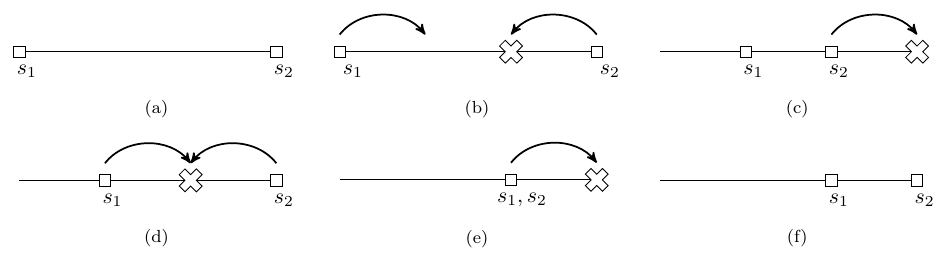
\includegraphics[width=0.8\textwidth]{images/k-server-double-coverage.png}
    \caption{k-Server: $DoubleCoverage$ anhand von $Greedys$ worst-case Beispiel}
    \label{k-server-double-coverage}
\end{figure}

\begin{algorithm}[h]
\caption{Double Coverage (ein Zeitschritt)}
\begin{algorithmic}
    \State $s \gets x_i$
    \State $s_{rechts} \gets \lambda; s_{links} \gets \lambda$
    \State $s_{rechts} \gets $ Server direkt rechts neben $s$
    \State $s_{links} \gets $ Server direkt links neben $s$
    \If{$s_{rechts} = \lambda$}
        \State output "Bewege $s_{links}$ zu $s$"
    \ElsIf{$s_{links} \gets \lambda$}
    \State output "Bewege $s_{rechts}$ zu $s$"
    \Else
    \State $d \gets \min \{ \dist(s_{rechts} , s), \dist(s_{links} , s) \}$
    \State output "Bewege $s_{rechts}$ um $d$ nach links und $s_{links}$ um d nach rechts"
    \EndIf
\end{algorithmic}
\end{algorithm}

\paragraph{Satz}
$DoubleCoverage$ ist k-kompetitiv für k-Server auf $\M_{[0,1]}$.

\underline{Beweis}:
Siehe Skript S.49ff.

Ziel: Definiere Potentialfunktion $\Phi$ so dass die Bedingungen vom Satz gelten.
\\
Sei $K_{DC} = \{p_1^{DC}, \dots , p_k^{DC}\}$ eine Konfigurationen von DC (d.h. die Positionen seiner Server).
Sei $K_{Opt}$ analog.
Seien $M_{\min} (K_{DC}, K_{Opt})$ die Kosten eines minimalen Matchings
und sei $DC(K_{DC})$ die Summe der paarweisen Distanzen aller Server von DC.
Wir definieren:
$$\Phi (K_{DC}, K_{Opt}) := k \cdot M_{\min} (K_{DC}, K_{Opt}) + DC(K_{DC}) $$

Beobachte: $\Phi$ ist positiv, konstant, und hängt nicht von $n$ ab. Konkret (Bedingung 1):
\footnote{Recall that wir uns in $\M_{[0,1]}$ bewegen, d.h. alle Distanzen zwischen zwei Punkten sind $\leq 1$.}
$$ 0 \leq \Phi (K_{DC}, K_{Opt}) \leq k \cdot k + \binom{k}{2} \leq 2 k^2 := \beta $$

Zeige nun dass $\forall i$ gilt $(\star)$:
$ \Phi(x_i) - \Phi(x_{i-1}) \leq k \cdot cost(Opt(x_i)) - cost (DC(x_i)) $ (Bedingung 2).
\\
Schätze dazu ab wie sich das Potential verändert (durch die Änderung der Konfiguration)
wenn erst $Opt$ und dann $DC$ einen Zug machen.

Der Zug von $Opt$ vergrössert $\Phi$ um $\leq k \cdot cost(Opt(x_i))$
(maximal ein Server wird um $cost(Opt(x_i))$ bewegt, nur $k \cdot M_{\min}$ ist affected).

Der Zug von $DC$ verändert $\Phi$ um:
\begin{itemize}
    \item[Fall 1:] $x_i$ ist ``ganz aussen''. OBdA wird $s_{rechts}$ nach links verschoben.
        Der zweite Summand vergrössert das Potential um $\leq (k-1) \cdot cost(DC(x_i))$.
        \\
        OBdA existiert ein minimales Matching das $s$ (von $Opt$ bereits nach $x_i$ bewegt)
        und $s_{rechts}$ matched -- siehe Fallunterscheidung).
        D.h. die Kosten von $k \cdot M_{\min}$ verringern sich um $k \cdot cost(DC(x_i))$.
        \\
        $\implies$ insgesamt gilt $(\star)$
    \item[Fall 2:] $x_i$ ist zwischen $s_{links}$ und $s_{rechts}$.
        Der zweite Summand wird um $cost(DC(x_i))$ kleiner (da sich $s_{links}, s_{rechts}$ näher kommen).
        OBdA sind vor dem Zug von $DC$ $s$ und $s_{links}$ (oder $s$ und $s_{rechts}$) gematched.
        Dies verringert die Kosten von $M_{\min}$ um $cost(DC(x_i))/2$.
        \\
        Der andere wird mit einem $s'''$ von $Opt$ gematched.
        Hier erhöhen sich die Kosten um $\leq cost(DC(x_i))/2$.
        D.h. der erste Summand bleibt gleich oder wird kleiner.
        \\
        $\implies$ insgesamt gilt $(\star)$
\end{itemize}
$\implies$ Bedingung 1 + 2 vom Satz erfüllt $\implies$ $DC$ ist k-kompetitiv.

\newpage

\end{document}
